\subparagraph*{Difference Estimation Sampling}

Problemi tipici che bisogna indirizzare è la media e la deviazione standard.
La \textbf{media} non è un fenomeno che cattura bene l'andamento generale, per la
presenza di \textit{outlier}, ovvero dei punti fuori dal comportamento
tipico del campione.
La media è un parametro poco affidabile (va verificato ulteriormente). Un
parametro più affidabile che non è soggetto agli
outlier è la \textbf{mediana}.

L'intervallo di confidenza è la probabilità che il campione rappresenti la parte
della popolazione. Viene rappresentato con un $\epsilon$, il quale più piccolo è e
meglio è. Solitamente, si usa un intervallo di confidenza del 90\%. Un problema
è la possibilità di usare una distribuzione fallace completamente duale rispetto
all'intervallo di confidenza.


\subparagraph*{Tipi di campionamento}

\subsubparagraph*{Campionamento Stop-or-Go} facciamo un campionamento ridotto, se trovo
ciò che cerco mi fermo (e.g. se i primi 20 elementi hanno zero errori allora mi fermo,
altrimenti...).

\subsubparagraph*{Campionamento discovery:} usato quando l'occorrenza dell'evento che
sto cercando è molto rara.

\subsubparagraph*{Campionamento degli attributi:} un attributo è qualsiasi
caratteristica che identifica una transazione rispetto alle altre (es.
transazioni effettuate ad un certo orario).\\
\newline
\textbf{Tasso di errore tollerabile:} il massimo rate di errore
tollerabile.\\
\newline
\textbf{Campionamento variabile:} quanto è accurato il campione nel rappresentare
l'intera popolazione?


\subparagraph{Campionamento variabile}

Si guardi la figura \ref{fig:variable:sampling}.

\begin{figure}[h!]
        \begin{center}
                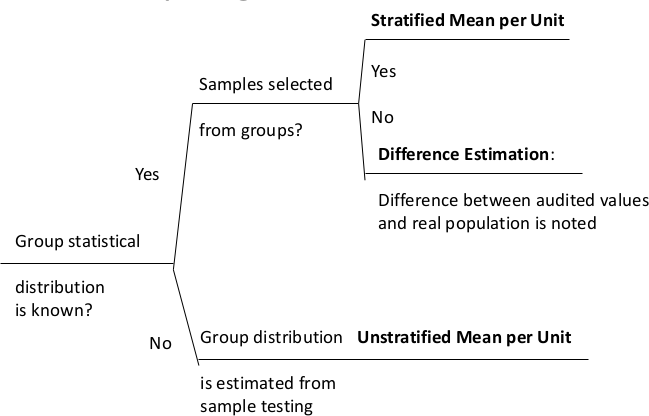
\includegraphics[scale=0.5]{res/img/variable_sampling.png}
        \end{center}
        \caption{Procedimento per il campionamento variabile.}
        \label{fig:variable:sampling}
\end{figure}

\subsubparagraph*{Generic Audit Software (GAS)}

Questa tipologia di tool sono molto utili e danno la possibilità di avere
accesso a:
\begin{itemize}
\item Accesso degli utenti ai file;
\item Organizzazione dei file;
\item Selezione dei dati (eg. selezione di un insieme di record);
\item Funzioni statistiche;
\item Funzioni aritmetiche.
\end{itemize}

\subsection{Step 8: Preparare il rapporto di Audit}

È importante identificare:
\begin{itemize}
\item Chi deve ricevere il rapporto?
\item Contesto (cosa viene analizzato), gli obiettivi, il periodo coperto e
quanto l'audit è durato\footnote{Audit che durano troppo poco con tante persone
da analizzare non vanno bene, soprattutto se devono essere svolti in poco
tempo.};
\item Findings (quello che è stato trovato), che deve essere supportato da delle
\emph{evidence} (prove). Le raccomandazioni possono essere date in due modi:
seguendo gli standard (es. standard ISO) o mettendo assieme la nostra
esperienza, la nostra conoscenza e quello che può fare l'azienda per risolvere i
problemi evidenziati;
\item Raggruppare per concretezza delle evidenze che abbiamo trovato;
\item Menzionare i problemi trovati e le critiche costruttive.
\end{itemize}

Il rapporto di audit è una parte molto importante: un rapporto dettagliato
permette ai successori di verificare il corretto funzionamento o meno
dell'azienda negli anni passati e permette di capire meglio il contesto. Un
rapporto di audit dovrebbe essere bilanciato, altrimenti se si arriva a mettere
a fuoco troppe cose negative non va bene, ma è importante anche non trascurarle.
È importante tenere a mente che il rapporto di audit è fatto per essere letto
dai ``piani alti''. Tenersi alle prove e ai fatti è sempre un'azione
consigliata.

\subsubsection{Evidenza}

Sono delle prove e esistono in diverse forme: note dalle interviste, risultati
dei test, email o corrispondenza, documentazione e osservazioni.

Le migliori fonti per ottenere informazioni sono:
\begin{itemize}
\item \textbf{Esterne:} fonti da organizzazioni esterne (es. i fornitori);
\item \textbf{Qualificate:} le più autorevoli;
\item \textbf{Oggettive:} evidenze per cui non è possibile esprimere un periodo
soggettivo
\item \textbf{Tempo:} deve essere coerente con il periodo della nostra attività
di audit
\end{itemize}

\subsubsection{Comunicazione dei risultati}

La comunicazione dei risultati è una passo decisivo. Questi risultati devono
essere riportati alle persone interessate.
La parte grossa dell'audit deve essere consegnata ai manager ad alto
livello.

\begin{figure}[h!]
        \begin{center}
                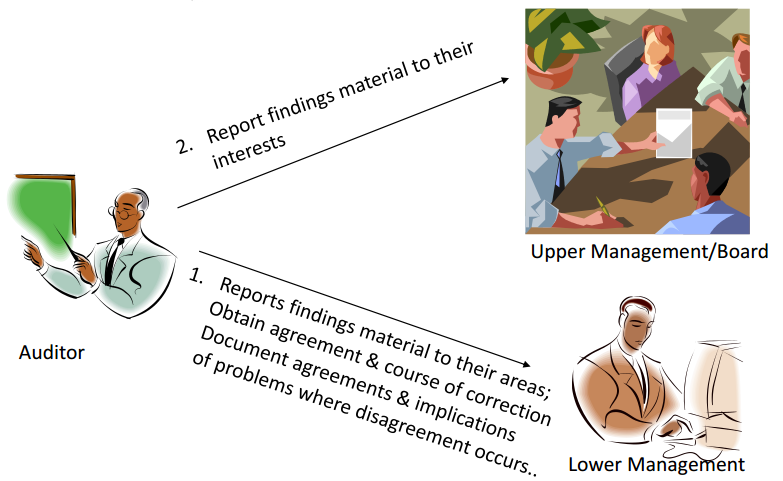
\includegraphics[scale=0.4]{res/img/communication_audit.png}
        \end{center}
        \caption{Procedimento per la comunicazione dei risultati dell'audit.}
\end{figure}

\subsection{Step 9: Prosieguo}


Il \textit{follow-up} serve a verificare se il management ha intrapreso le azioni
necessarie a correggere i problemi in tempo.

\section{Raccomandazioni finali sull'Audit}

Queste ultime note sono molto importanti e vanno sempre tenute in
considerazione:
\begin{itemize}
\item Mai eccedere lo scopo di quello che si deve fare, ovvero mai ficcare il
naso dove non serve. I permessi che vengono accordati devono essere messi per
iscritto, affinché ne rimanga una traccia.
\item Tutti i test potrebbero impattare sul sistema quindi è una buona
pratica avvisare i settori interessati dei possibili disservizi prima di eseguire
qualsiasi test.
\item Quando si lavora con i dati è importante non toccare dati o configurazioni
importanti.
\end{itemize}


\section{Tipi di audit}

Audit finanziario (assicura l'integrità degli asset finanziari),
operazionale (valuta i controlli interni per uno specifico processo/area),
integrativo (sia finanziario che operazionale), forense (è successo un evento
negativo che ha scatenato reazioni civili o penali e viene chiamato un auditor
esterno per fare analisi forense), IS (IS sta salvaguardando i dati, fornisce
CIA in un modo efficiente), amministrativo (verifica l'efficienza dei processi
e dell'organizzazione).

\subsection{Computer-Assisted Audit Techniques (CAAT)}

I software permettono agli auditor di:
\begin{itemize}
\item Accedere e analizzare i dati nel database;
\item Effettuare test di compliance;
\item Effettuare penetration test;
\item Testare le applicazioni.
\end{itemize}


\subsection{Controllare l'auto-valutazione}

Sistema di audit interno che migliora l'audit esterno. I benefici consistono
nel fatto che si lavora con le persone e questo serve per insegnare ai
dipendenti e dare una migliore immagine dell'azienda.


\subsection{Service Learning Component: Non-Disclosure Agreement}

Supponiamo che si sia una situazione del genere:

\begin{verbatim}
You: I developed an audit plan for Help-The-Community
Interviewer: What specifically did you do?
You: We tried to break into their wireless network
Interviewer: What did you find?
You: They had no security. They were hopelessly non-technical.
Their password was `HelpTheCommunity', and transmissions were
unencrypted. I could read everything...
\end{verbatim}

In questo dialogo, è evidente come ci sia un rilascio di informazioni non
controllato, che potrebbe portare un attacco di tipo malizioso.

Il problema è che l'intervistato ha divulgato informazioni sull'azienda,
nonostante il NDA. Anche se i problemi fossero attualmente risolti sta comunque
infangando il nome della società sotto audit.


Un comportamento corretto potrebbe essere:
\begin{verbatim}
You: I developed an audit plan for Help-The-Community
Interviewer: What specifically did you do?
You: We did a penetration test. However, I signed a
non-disclosure agreement, so I am not at liberty to
say specifically what we did or found.
Interviewer: Were you successful in breaking in?
You: I can't say. However, if you would like to contact my
community partner as a reference, here is her contact
information...
\end{verbatim}

\section{Esercizi}
Gli esercizi su questa parte si trovano in \ref{EsAudit}.

%ESERCIZI

% Ho lasciato qui i commenti degli esercizi perché c'è una nota che non so dove
% posizionarla, quindi così riusciamo a capire che numero di esercizio è riferito
% quella nota contando il numero di ``Altro esercizio'' qui scritti!

% Altro esercizio



% Altro esercizio


%Altro esercizio


%Altro esercizio

%Altro esercizio

%Altro esercizio

%Altro esercizio

% RISCHIO DI CONTROLLO = QUANDO IL CONTROLLO FALLISCE -> Per mitigarlo si usano
% controlli compensativi

%Altro esercizio

%Altro esercizio
